\documentclass[conference]{IEEEtran}
\IEEEoverridecommandlockouts

\usepackage{amsmath}
\usepackage{amssymb}
\usepackage{booktabs}
\usepackage{url}
\usepackage{graphicx}
\usepackage{tikz}
\usetikzlibrary{arrows.meta,positioning,shapes.geometric}

\title{From URDF to Current Control: A Framework for Safety-Constrained Autonomous Commissioning of Robot Manipulators}

% ICRA 2027 uses double-anonymous review. Replace only after review.
\author{Anonymous Authors}

\begin{document}
\maketitle

\begin{abstract}
Commissioning a geared manipulator for direct teaching requires more than a
gravity law: an engineer must verify actuator polarity, choose collision-free
and informative motions, determine which parameters are observable, calibrate
current-to-torque behavior, validate the result, and switch control modes
safely. This paper formulates a description-driven framework designed to automate
these steps from a URDF and a minimal actuator-capability description. The
kinematic structure, limits, and collision geometry are trusted, whereas link
dynamics and raw-current scaling need not be. The framework constructs a safe
configuration set, verifies hardware sign mappings, and selects each
calibration motion as a safety-constrained epistemic action that reduces model
uncertainty. It identifies either a current-domain compensation map or
physical gravity base parameters after independent torque-scale calibration,
performs bidirectional friction sweeps, and enables current control only after
held-out validation. We instantiate the current-domain identification and
deployment stages on a six-degree-of-freedom DYNAMIXEL arm in ROS~2. A 181-s
physical all-axis run yields chronological held-out raw-current $R^2$ values of
0.869, 0.952, and 0.956 for the three gravity-supported axes. Preliminary
signed-current commissioning verifies the command path and exposes why a
retained position loop remains stiff for hand guiding. These results establish
feasibility of the sensing, fitting, and deployment path; autonomous safe-space
generation, calibrated physical identification, and cross-morphology trials
remain to be completed.
\end{abstract}

\begin{IEEEkeywords}
autonomous commissioning, robot dynamics identification, experiment design,
gravity compensation, current control, direct teaching
\end{IEEEkeywords}

\section{Introduction}
Direct teaching allows an operator to program a manipulator by physically
guiding it. Low-cost geared arms are attractive leader devices, but they are
normally commissioned through a robot-specific sequence of manual steps:
check encoder and motor signs, select a safe pose, tune an excitation, fit a
model, decide which joints to compensate, and finally change from a stiff
position servo to a torque-like control mode. An error in any step can make the
arm difficult to move or, more seriously, command gravity current with the
wrong sign.

Existing gravity and friction identification methods solve important pieces of
this problem \cite{Chen2018,Chen2023}, and mature dynamic-identification work
already provides observability analysis and informative trajectory design.
The unresolved systems question considered here is how to connect those pieces
into a validation-gated commissioning procedure that begins with a robot
description and actuator feedback rather than a hand-tuned experiment.

We assume that the URDF kinematic tree, joint axes, limits, and collision
geometry are available, but its inertial properties are missing or inaccurate.
A hardware adapter exposes position and current-control capabilities, encoder
state, raw present current, and actuator limits. Thus, the method is
\emph{URDF-guided}, not model-free. Its desired user interface is a URDF plus a
hardware configuration; joint order, excitation, identifiable parameter set,
and validation decision are generated by the system.

The unifying view is that calibration is not merely data collection after a
trajectory has been chosen. Each calibration motion is an
\emph{information-seeking physical action}: the robot decides what safe action
to execute next in order to reduce uncertainty in its own compensation model.
This epistemic-action view connects geometric safety, parameter observability,
experiment design, and the decision to deploy or request more evidence.

For slowly guided motion, the actuator torque is approximated by
\begin{equation}
 \tau_m \simeq g(q) + r(\dot{q}),
 \label{eq:quasistatic}
\end{equation}
where $q$ and $\dot{q}$ are joint position and velocity, $g(q)$ is gravity
torque, and $r(\dot{q})$ is drivetrain friction. This approximation neglects
inertia, centrifugal, and Coriolis terms; it is appropriate only for the
low-speed direct-teaching task considered here.

The key distinction is between predicting compensation current and recovering
physical parameters. Current feedback alone can identify a useful
\emph{current-domain} map, but it cannot in general separate motor torque scale
from mass and center-of-mass parameters. A known calibration load or other
independent torque reference is required for physical identification. The
framework makes this ambiguity explicit rather than labeling raw current as
joint torque.

The contributions of the present framework and preliminary study are:
\begin{enumerate}
  \item A formal commissioning pipeline that combines URDF-derived safety
  constraints, paired actuator-polarity verification, observability analysis,
  and safety-constrained epistemic action selection, followed by held-out
  validation and safe controller activation.
  \item A two-level identification formulation: per-joint current-domain
  compensation when actuator scale is unknown, and observable physical gravity
  parameters when an independent calibration load anchors that scale.
  \item An observability-guided subtree schedule and a separate bidirectional
  velocity-sweep stage for friction, replacing a fixed distal-to-proximal rule
  and preventing exact mass/CoM claims when only base-parameter combinations
  are observable.
  \item A preliminary OM6DOF instantiation demonstrating the current logging,
  chronological held-out fitting, and safety-limited signed-current deployment
  stages, together with a protocol for completing autonomy and scalability
  experiments.
\end{enumerate}

\section{Related Work and Positioning}
Gravity compensation may be learned without a geometric model \cite{Yu2018},
while direct zero-moment teaching with self-measured gravity and friction has
already been demonstrated in current control \cite{Chen2018,Chen2023}. Hence,
neither the quasi-static law nor signed-current hand guiding is claimed as new.
Recent zero-force drag work also combines minimum gravity parameters, nonlinear
friction identification, current feedback, and start-up compensation
\cite{Li2025ZeroForce}.
Nonlinear disturbance modeling on the dVRK further shows why direction,
workspace, and payload validation are necessary \cite{Lin2019}; full dynamic
identification targets a broader regime than the slow teaching task considered
here \cite{Zhou2026}.

Base-parameter computation and optimal robot excitation are established topics
\cite{Gautier1991Base,Swevers1997Optimal}. Backward sequential identification
has also explicitly used a distal-to-proximal structure \cite{Jung2018Backward},
so distal scheduling is not a novelty claim. FIGAROH is particularly close to
the broader direction of this paper: it constructs identification models from
robot descriptions and supports observability, constrained experiment design,
estimation, and validation \cite{Nguyen2023FIGAROH}. AURT similarly automates
important dynamics-calibration steps \cite{Madsen2022AURT}. Provably safe
online identification and virtual-constraint excitation design provide stronger
safety treatments than the monitored constraints presently proposed here
\cite{Tian2024VirtualConstraints,Zhang2025SafeSysID}.

Table~\ref{tab:related_work} therefore locates the remaining integration target:
hardware qualification, explicit separation of raw-current and physical
parameters, staged low-speed gravity/friction experiments, and a validation-
gated switch into direct-teaching current control. The present results cover
only a preliminary subset of that target.

\begin{table*}[t]
\caption{Positioning of the proposed commissioning framework.}
\label{tab:related_work}
\centering
\footnotesize
\begin{tabular}{p{30mm}p{61mm}p{69mm}}
\toprule
Line of work & Established capability & Boundary addressed here \\
\midrule
Current direct teaching \cite{Chen2018,Chen2023,Li2025ZeroForce} & Gravity/friction current identification and zero-force control. & Commissioning raw-current actuators from a description and guarding mode activation. \\
Dynamic identification \cite{Gautier1991Base,Swevers1997Optimal,Jung2018Backward} & Base parameters, informative excitation, and sequential subtree estimation. & Capability-aware choice of which experiment is both informative and deployable. \\
Calibration toolchains \cite{Nguyen2023FIGAROH,Madsen2022AURT} & Description-driven model construction, constrained excitation, fitting, and validation. & Current/physical ambiguity, polarity checks, staged friction, and direct-teaching handoff. \\
Safe/constrained ID \cite{Tian2024VirtualConstraints,Zhang2025SafeSysID} & Constrained excitation and formal safe online identification. & Conservative hardware monitors and explicit evidence gates; no formal safety claim yet. \\
This paper & Complete framework formulation; preliminary current-domain OM6DOF instance. & Autonomous experiment generation, physical calibration, and cross-robot evidence remain open. \\
\bottomrule
\end{tabular}
\end{table*}

\section{Commissioning Problem Formulation}
For an $n$-joint robot, the actuator-side dynamics are
\begin{equation}
 \tau_m=M(q)\ddot q+C(q,\dot q)\dot q+g(q)+\tau_f(\dot q)+\tau_{\rm ext}.
 \label{eq:dynamics}
\end{equation}
Direct-teaching commissioning uses contact-free, low-acceleration experiments,
so $\tau_m\simeq g(q)+\tau_f(\dot q)$. Contact by any link other than the fixed
base would add $J_c^TF_c$ and invalidate this separation; a mechanical support
may therefore be used for activation and polarity checks, but not during model
measurements.

The raw current observation $u\in\mathbb R^n$ is modeled as
\begin{equation}
 u=A\tau_m+b+\eta,\quad A=\operatorname{diag}(s_1a_1,\ldots,s_na_n),
 \label{eq:current_observation}
\end{equation}
where $a_i>0$ is an assembled-joint raw-current/torque magnitude,
$s_i\in\{-1,+1\}$ is hardware polarity, $b$ is bias, and $\eta$ includes servo
and sensing error. If $A$ and the link dynamics are both unknown, current and
encoder data do not uniquely determine either one; for example,
$AY_g\pi_g=(cA)Y_g(\pi_g/c)$ for any $c>0$. The
commissioner consequently supports two outputs: (i) a current-domain map
$\hat u_g(q)+\hat u_f(\dot q)$ sufficient for bounded compensation, and (ii) a
physical gravity model only when an independent load or torque reference
anchors $A$.

Inputs are the URDF topology, transforms, limits, and collision geometry; an
actuator adapter declaring control modes, feedback fields, and current limits;
and a minimal world description containing the base mounting surface. URDF
inertial values are treated as optional priors, not ground truth.

\begin{figure*}[t]
\centering
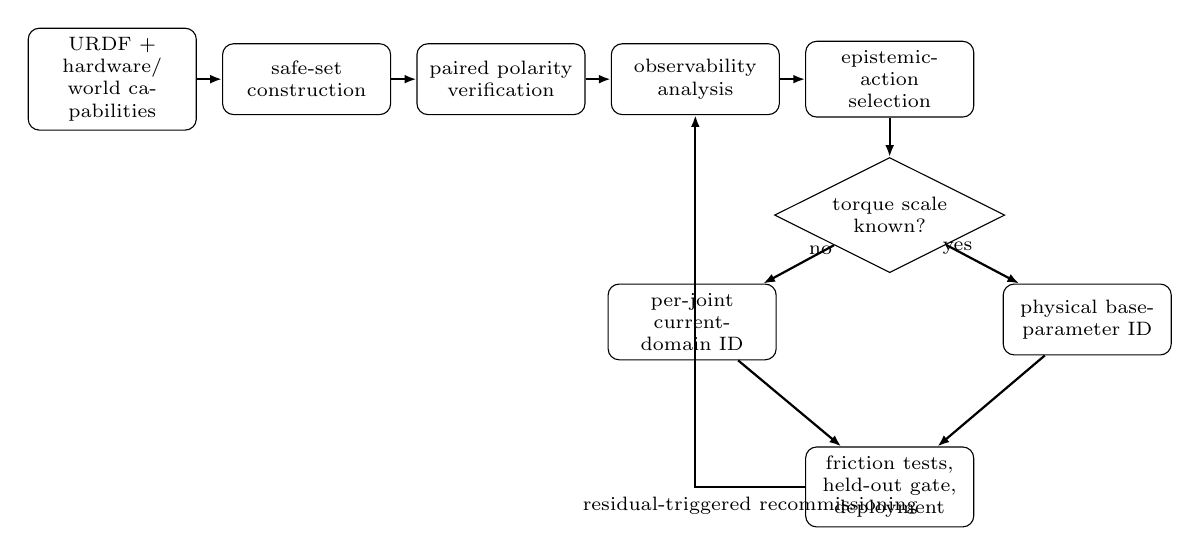
\begin{tikzpicture}[font=\scriptsize, node distance=3.2mm,
  block/.style={draw, rounded corners, align=center, minimum height=9mm,
                text width=19mm},
  decision/.style={draw, diamond, aspect=2.0, align=center,
                   inner sep=0.7mm, text width=16mm},
  arrow/.style={-{Latex[length=1.5mm]}, thick}]
\node[block] (input) {URDF + hardware/\\world capabilities};
\node[block, right=of input] (safe) {safe-set\\construction};
\node[block, right=of safe] (sign) {paired polarity\\verification};
\node[block, right=of sign] (obs) {observability\\analysis};
\node[block, right=of obs] (design) {epistemic-action\\selection};
\node[decision, below=5mm of design] (scale) {torque scale\\known?};
\node[block, below left=5mm and 7mm of scale] (current) {per-joint current-\\domain ID};
\node[block, below right=5mm and 7mm of scale] (physical) {physical base-\\parameter ID};
\node[block, below=22mm of scale] (gate) {friction tests,\\held-out gate,\\deployment};
\draw[arrow] (input) -- (safe);
\draw[arrow] (safe) -- (sign);
\draw[arrow] (sign) -- (obs);
\draw[arrow] (obs) -- (design);
\draw[arrow] (design) -- (scale);
\draw[arrow] (scale) -- node[above right]{no} (current);
\draw[arrow] (scale) -- node[above left]{yes} (physical);
\draw[arrow] (current) -- (gate);
\draw[arrow] (physical) -- (gate);
\draw[arrow] (gate.west) -| node[pos=.25,below]{residual-triggered recommissioning} (obs.south);
\end{tikzpicture}
\caption{Proposed autonomous commissioning loop. Safe calibration motions are
epistemic actions selected to reduce uncertainty. Unknown torque scale routes
the system to independent per-joint current-domain maps; only calibrated scale
permits shared physical base-parameter and subtree reasoning. Both branches
must pass friction and held-out deployment gates.}
\label{fig:architecture}
\end{figure*}

\section{Proposed Autonomous Commissioning Framework}
\subsection{Safety Set and Hardware Verification}
With joint-limit margin $m_q$, self/environment clearance $d_{\min}$, and a
known base mounting plane, the geometric safe set is
\begin{equation}
 \begin{aligned}
 \mathcal Q_{\rm safe}=\{q\mid{}&q^-+m_q\le q\le q^+-m_q,\\
                         &d_{\rm self}(q),d_{\rm env}(q)\ge d_{\min}\}.
 \end{aligned}
 \label{eq:safe_set}
\end{equation}
Candidate paths must also satisfy velocity, acceleration, current, temperature,
and tracking-error limits. Because current demand is initially unknown, the
last constraints cannot be guaranteed from geometry alone. Execution therefore
begins with conservative envelopes and expands them only while online monitors
remain below abort thresholds.

The URDF specifies positive joint direction, but the mapping from signed
current to encoder direction may be wrong in the hardware configuration. For a
supported joint, paired pulses estimate
\begin{equation}
 s_i=\operatorname{sgn}\!\left(
 \frac{\Delta q_i(+u_\epsilon)-\Delta q_i(-u_\epsilon)}{2u_\epsilon}\right).
 \label{eq:polarity}
\end{equation}
Pulse magnitude is increased only until displacement exceeds an encoder
threshold or a conservative current cap is reached. Pairing reduces first-order
gravity drift; displacement, time, and communication watchdogs remain active.
This verifies actuator polarity, not the URDF joint axis.

\subsection{Observability and Experiment Selection}
Gravity is linear in link mass and first moments,
\begin{equation}
 g(q)=Y_g(q)\pi_g,
 \label{eq:gravity_regressor}
\end{equation}
where each link contributes $[m_i,m_ic_{ix},m_ic_{iy},m_ic_{iz}]$. Stacking
candidate measurements gives $\mathcal Y_g$. Its singular-value decomposition
$\mathcal Y_g=U\Sigma V^T$ defines numerical rank $r$ and the observable base
parameters $\beta_g=V_r^T\pi_g$; components in the null space are not reported
as individual mass or center of mass.

Before computing numerical rank, the regressor is noise-whitened and its
columns are normalized; otherwise mixed mass and first-moment units make
singular values and condition numbers arbitrary. If gravity, friction, and bias
are estimated together, observability is evaluated on the augmented regressor,
not $\mathcal Y_g$ alone.

The next safe experiment $e$ is selected from candidate poses or trajectories
by an incremental information--risk objective,
\begin{equation}
 e^*=\arg\max_{e\in\mathcal E_{\rm safe}}
 \left[\log\frac{\det(F_{\rm prev}+F_e+\lambda I)}
 {\det(F_{\rm prev}+\lambda I)}-\lambda_R R(e)\right],
 \label{eq:experiment_design}
\end{equation}
where $F_e$ is the normalized regressor information matrix and $R(e)$ penalizes
clearance, current, and tracking risk. A Fourier, multisine, or spline path is
only the trajectory parameterization; its amplitudes, frequencies, and joint
participation are outputs of (\ref{eq:experiment_design}).
Thus, $e^*$ is an epistemic action rather than a predetermined calibration
motion: its physical purpose is to reduce the model uncertainty that currently
blocks a validation decision, subject to the admissible safety envelope.

For joint $i$, gravity contains contributions from its descendant subtree,
\begin{equation}
 \tau_{g,i}=\sum_{\ell\in\mathcal D(i)}Y_{i\ell}(q)\pi_\ell.
 \label{eq:subtree}
\end{equation}
A calibrated, observable distal subtree can be subtracted before estimating a
parent only in physical mode, where all joints share consistent torque units.
Per-joint current-domain coefficients cannot be propagated as link parameters.
Moreover, a distal joint may have zero gravity sensitivity or expose only one
parameter combination. We therefore use \emph{observability-guided
subtree scheduling}: distal-first is preferred when it increases rank at low
risk, but it is not imposed as a universal identification rule.

\subsection{Current Scale, Gravity, and Friction}
The observability stage branches according to whether the actuator torque scale
has an independent physical anchor. The two branches produce different kinds
of knowledge and must not be merged implicitly.
Without an independent torque reference, each joint is fitted directly in the
command domain,
\begin{equation}
 u_i=\phi_{g,i}(q)^T\theta_{g,i}+u_{f,i}(\dot q_i)+b_i,
 \label{eq:current_domain}
\end{equation}
where $\phi_{g,i}$ contains the nonzero, SVD-reduced kinematic columns of the
$i$th gravity-regressor row. Thus, $\theta_{g,i}$ is described only as an
effective current-domain parameter; it supports per-joint compensation but not
physical descendant-subtree propagation. For physical identification, a
payload of measured mass and center of mass is attached at a known transform. Matched
loaded and unloaded measurements give \cite{Gautier2012DriveGains}
\begin{equation}
 \Delta u=A\Delta g_p(q),\qquad
 \Delta g_p(q)=\frac{\partial V_p(q)}{\partial q},
 \label{eq:payload_scale}
\end{equation}
which estimates the observable entries of $A$. Axes receiving negligible
payload torque require a different load orientation or an external torque
reference. With $A$ anchored, robust least squares estimates only the base
parameters supported by the SVD analysis.

Friction is identified after gravity using constant-speed passes through the
same configurations in both directions, after trimming acceleration segments.
Outside a stiction dead zone,
\begin{equation}
 \tau_{f,i}(v)=
 \begin{cases}
 f_{c,i}^{+}+f_{v,i}^{+}v,&v>v_\epsilon,\\
 -f_{c,i}^{-}+f_{v,i}^{-}v,&v<-v_\epsilon.
 \end{cases}
 \label{eq:friction}
\end{equation}
with nonnegative $f_c^{\pm}$ and $f_v^{\pm}$.
At matched position and speed magnitude, the half-sum of positive/negative
measurements emphasizes gravity, while their half-difference emphasizes odd
friction. This staged experiment is preferred to interpreting a quantized
multisine velocity trace as a final friction measurement.

\subsection{Validation-Gated Deployment}
The model is tested on unseen configurations, velocity directions, and a
separate payload condition. The gate checks current-prediction error, released
pose drift, saturation frequency, temperature, polarity, and fault response.
Physical transparency additionally requires a handle-force measurement. Let
$\gamma_i$ be one only when polarity, rank, confidence interval, held-out
error, Mode~0 transfer, and actuator/fault tests pass. Deployment also requires
the uncertainty envelope
\begin{equation}
 |\mu_{u,i}(q)|+k\sigma_{u,i}(q)\le u_{\mathrm{safe},i}
 \quad\forall q\in\mathcal Q_{\mathrm{deploy}}.
 \label{eq:validation_gate}
\end{equation}
The command applies $\Gamma=\operatorname{diag}(\gamma_i)$ before saturation
and slew limiting. A failed gate blocks free Mode~0 activation and requires a
mechanically supported state or safe handoff to position control; zero current
alone is not safe for an unsupported gravity-loaded arm. Residual-triggered
recommissioning is evaluated only during declared contact-free self-checks or
tool-change events, because human teaching force is itself a residual.

\section{Preliminary OM6DOF Instantiation}
\subsection{Platform and Existing Excitation}
The preliminary platform is a six-DOF vertical OM6DOF arm driven by
XM430-series DYNAMIXEL actuators \cite{RobotisXM430} through ROS~2 Humble and
\texttt{ros2\_control} \cite{ROS2Control}. Its effort state is raw Present
Current, not measured joint torque. The deployed controller evaluates a KDL
gravity prior and folds gripper/camera branches into the nearest chain link.
The configured 0.114-kg distal mass includes an unmeasured 0.08-kg
camera/bracket estimate. Offline analysis instead finite-differences the
potential energy of the expanded URDF tree. Numerical equivalence of these two
gravity implementations remains to be verified.

The existing \texttt{teaching\_all} data are a manually configured precursor,
not output of the complete autonomous experiment designer. Each joint followed
three sinusoidal terms,
\begin{equation}
 q_i(t)=q_{i,0}+\sum_{k=1}^{3}A_{ik}\sin(\omega_k t),
 \label{eq:multisine}
\end{equation}
at 0.5, 0.8, and 1.2~rad/s, within manually checked joint-limit margins. The
run contains 18,156 samples over 181.05~s at 100.27~Hz. It was executed under
the position trajectory controller; transferring its effective current model
to signed Current Control is therefore an explicit assumption.

Figure~\ref{fig:multisine_motion} shows the three axes retained for preliminary
gravity support. Reported velocity is quantized in approximately
0.02397-rad/s increments. $T_g^{\mathrm{URDF}}$ is a nominal model prediction,
and Present Current is a raw register value.

\begin{figure*}[t]
\centering
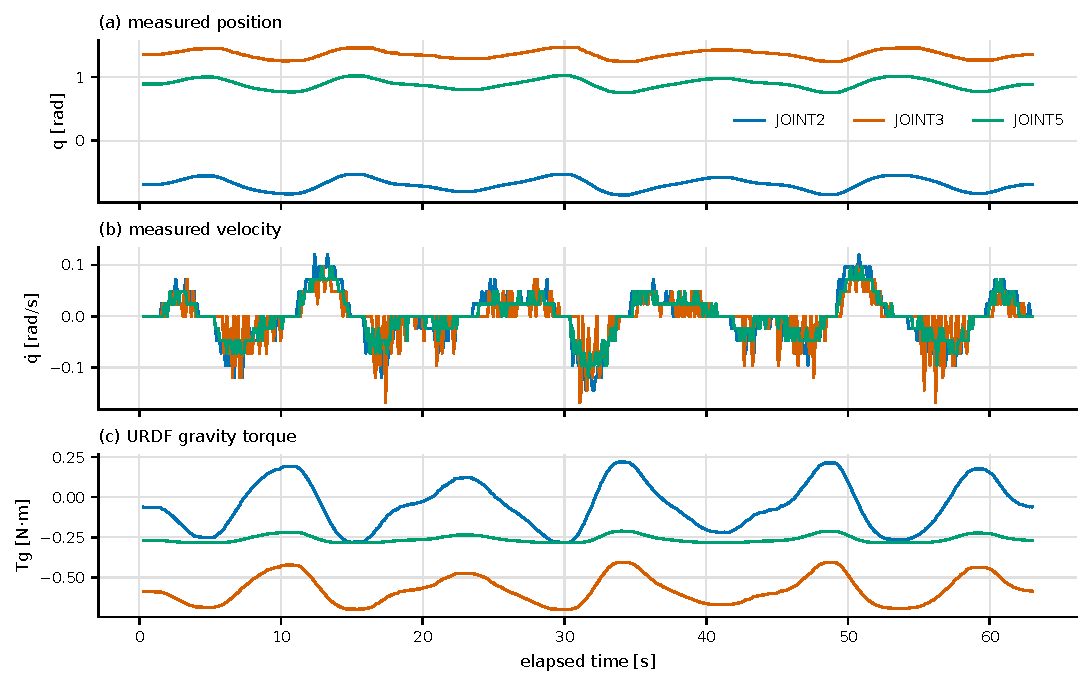
\includegraphics[width=\textwidth]{figures/multisine_motion_measurements.pdf}
\caption{Existing OM6DOF multisine data over the first 63~s. Position and
reported velocity are measured; $T_g^{\mathrm{URDF}}$ is the whole-tree model
prediction. This is preliminary manually bounded excitation, not yet an
autonomously synthesized experiment.}
\label{fig:multisine_motion}
\end{figure*}

\subsection{Chronological Current-Domain Fit}
For this precursor data set, the nominal gravity feature is fitted as
\begin{equation}
 u_i=c_{g,i}g_i^{\rm URDF}(q)+c_{c,i}\tanh(\dot q_i/\epsilon)
      +c_{v,i}\dot q_i+b_i.
 \label{eq:regression}
\end{equation}
Here $c_g$ is raw current per \emph{nominal-model} Nm: it combines actuator
scale and URDF inertial error and is not a physical torque constant. Candidate
friction terms are used only for prediction and remain disabled in deployment.

Every tenth row is retained (1,816 samples); samples with
$|\dot q_i|<0.005$~rad/s and the first/final 2~s are omitted. Training uses
$[2,120)$~s, followed by a 2-s guard interval, and testing uses
$[122,179.3)$~s. This is an unseen time block of the same trajectory, not
workspace or payload generalization.

\begin{table}[t]
\caption{Chronological held-out raw-current prediction on the existing
OM6DOF run.}
\label{tab:fit}
\centering
\scriptsize
\begin{tabular}{@{}lccrr@{}}
\toprule
Joint & $g^{\rm URDF}$ [Nm] & $c_g$ [raw/nom. Nm] & RMSE & $R^2$ \\
\midrule
J2 & $[-0.282,\ 0.219]$ & 176.39 & 10.63 & 0.869 \\
J3 & $[-0.699,\ -0.404]$ & 165.54 & 9.67 & 0.952 \\
J5 & $[-0.283,\ -0.211]$ & 139.34 & 5.89 & 0.956 \\
\bottomrule
\end{tabular}
\end{table}

The other test $R^2$ values are 0.383 (J1), 0.526 (J4), and 0.263 (J6).
Selecting J2/J3/J5 was a conservative manual decision, not an automatic
observability gate. Figure~\ref{fig:heldout_current} shows the prediction. The
quantized velocity and position-loop data preclude interpreting $c_v$ as a
validated physical friction coefficient.

\begin{figure*}[t]
\centering
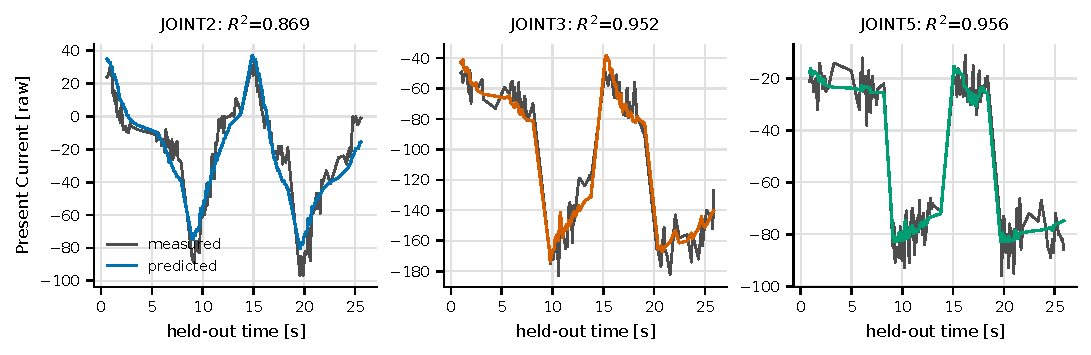
\includegraphics[width=\textwidth]{figures/multisine_heldout_current_fit.pdf}
\caption{Held-out Present Current prediction. Parameters use only
$[2,120)$~s; displayed test samples begin at 122~s. Both measured and predicted
quantities are raw current, not torque.}
\label{fig:heldout_current}
\end{figure*}

\section{Preliminary Signed-Current Deployment}
\subsection{Current-Based Position Control Baseline}
DYNAMIXEL Operating Mode~5 retains an internal position loop \cite{RobotisXM430}. In this mode,
Goal Current acts as a current ceiling rather than a signed torque command.
Experiments with a position setpoint plus a current limit produced a stiff,
non-smooth response. Reducing the position deadband made the arm sag, whereas
increasing it made the arm difficult to move. This trade-off is inherent to the
remaining position loop; on the present platform it did not provide transparent
hand guiding. A quantitative force comparison remains part of the final
evaluation.

\subsection{Pure Current Control}
The prototype teaching profile uses Operating Mode~0. The commanded current is
\begin{equation}
 u_i^{*}=\operatorname{sat}_{u_{\max,i}}
 \left(\hat u_{g,i}(q)+\hat u_{f,i}(\dot{q})+\hat b_i\right),
 \label{eq:command}
\end{equation}
where \texttt{sat} applies a symmetric current limit. The initial physical
trial uses $\hat u_{f,i}=0$ and $\hat b_i=0$, so that the gravity path and
activation behavior are validated before uncertain friction terms are
introduced. Full gravity--friction compensation is enabled only after
bidirectional constant-speed validation shows that these residual terms improve
held-out predictions and release drift. A 0.5-s current ramp and conservative
per-joint caps limit activation transients.

Unlike Mode~5, zero current is neutral in Mode~0. Consequently, the controller
does not hold a pose by itself; a supported arm, an active controller, current
limits, and a communication fail-safe are required. The normal position-control
stack and the teaching stack are mutually exclusive hardware owners.

\section{Preliminary Commissioning Results}
\label{sec:commissioning}
At a representative supported pose, the gravity model produced
$g_2(q)=0.1090$~Nm for joint~2. With the identified scale, the controller
commanded $19.38$ raw current ticks, while the measured present current was
18~ticks. This agreement verifies raw-current command tracking at that pose; it
does not verify physical gravity torque or identify actuator torque scale. The
arm was qualitatively more backdrivable than with the Mode~5 baseline. A small
residual joint-2 drift remained, indicating that bias, friction, gravity-model
error, or Mode~5-to-Mode~0 transfer error is still present.

These observations are gravity-only commissioning evidence, not a complete
gravity--friction performance evaluation. No interaction force, payload sweep,
temperature sweep, or repeatability statistic has yet been measured. The
current results therefore support feasibility of the deployment path but do not
establish general superiority over other hand-guiding methods or a validated
friction-compensation benefit. The Mode~0 spot check predates the chronological
reanalysis in Table~\ref{tab:fit}; it is not an independent validation of the
held-out fitted parameters.

\section{Evaluation Plan}
The existing experiment evaluates only current-domain prediction and a
single-pose deployment path. Table~\ref{tab:protocol} defines the measurements
needed to evaluate the complete framework. Unmeasured entries are protocols,
not claimed results. Each physical condition will be repeated at least three
times, with timestamped position, velocity, Goal Current, Present Current,
voltage, temperature, controller state, and hardware-fault status.

\begin{table}[t]
\caption{Evaluation matrix. Only the preliminary portion of RQ2 is currently
reported in Table~\ref{tab:fit}.}
\label{tab:protocol}
\centering
\scriptsize
\begin{tabular}{@{}p{11mm}p{23mm}p{28mm}@{}}
\toprule
Question & Comparison & Primary metrics \\
\midrule
RQ1 autonomy & manual vs. generated commissioning & interventions; completion; time \\
RQ2 information & manual, random-safe, and optimized excitation & rank; $\sigma_{\min}$; condition; held-out error \\
RQ3 safety & nominal and injected faults & clearance; peak current; abort latency \\
RQ4 transfer & 2/3/4/6-DOF and changed payload & success rate; residual; recovery \\
RQ5 teaching & Mode 5, nominal Mode 0, calibrated Mode 0 & handle force; drift; jerk; saturation \\
\bottomrule
\end{tabular}
\end{table}

RQ1 counts every user choice after the URDF, hardware adapter, and mounting
surface are supplied, including ready pose, joint order, parameter subset,
amplitude, and frequency. RQ2 first calibrates $A$ with a measured payload at
matched poses, then evaluates on a second payload and unseen workspace poses.
The optimized trajectory is compared with the existing manual multisine and a
safe random baseline using normalized regressors.

RQ3 records minimum collision distance in simulation and hardware current,
tracking, and watchdog aborts during bounded fault injection. RQ4 applies the
same software pipeline to modular 2-, 3-, 4-, and 6-DOF descriptions, then adds
a payload and measures residual detection and recovery after recommissioning.
RQ5 uses a calibrated handle load cell; subjective ease of motion is
supplementary only. Release drift and the RMS/95th-percentile jerk use identical
filters across controllers. Confidence intervals are computed by trial-level
bootstrap rather than treating adjacent time samples as independent.

\section{Safety and Reproducibility}
Changing DYNAMIXEL operating mode resets actuator settings; the procedure must
disable torque, write and verify zero Goal Current, start only one hardware
owner, and then enable the teaching controller with the arm supported. The
controller must command zero current upon deactivation or invalid state data.
Identification begins only after the support is removed and collision checks
confirm that no distal link contacts the mounting surface. Per-axis current and
slew caps, state timeouts, temperature limits, a dead-man input, and a physical
emergency stop remain outside the learned model.

For each submitted result, the expanded URDF, controller configuration,
firmware/model/ID register dump, supply voltage, payload, code commit, and raw
log will be archived. The candidate friction terms identified from multisine
data will be validated through bidirectional constant-speed sweeps independently
from the multisine run before they are enabled. The offline whole-tree and
deployed KDL gravity implementations must also agree numerically on the logged
configuration set before a physical-parameter result is reported.

\section{Limitations and Threats to Validity}
The full autonomous commissioner is a proposed framework; the current
implementation covers logging, predefined excitation, current-domain fitting,
and safety-limited deployment. It does not yet generate collision-free
experiments, perform payload-based torque calibration, or automatically gate
axes by observability. The manually selected multisine was collected under an
internal position servo, and velocity is quantized; transfer to Mode~0 and the
quasi-static assumption require dedicated validation.

Exact link masses and centers of mass are generally not individually
observable, and raw current cannot resolve their scale without an independent
load. Friction can vary with direction, temperature, supply voltage, and
gearbox history. The configured camera/bracket mass is unmeasured. Finally,
cross-morphology scalability and automatic recommissioning are research
hypotheses until RQ1--RQ4 are completed.

\section{Conclusion}
This paper formulates commissioning as the complete transition from a robot
description to validated current control, rather than as gravity fitting alone.
The framework combines safe-set construction, actuator-polarity verification,
observable-parameter analysis, information-driven experiment selection,
separate gravity/friction experiments, and a deployment gate. It also separates
current-domain compensation from physical identification so raw actuator
feedback is not mislabeled as torque. Existing OM6DOF data support feasibility
of the logging, held-out fitting, and signed-current command path, but not yet
the autonomy, physical accuracy, scalability, or friction benefit of the full
framework. The evaluation plan turns those gaps into explicit experiments for
the next revision.

\bibliographystyle{IEEEtran}
\bibliography{om6dof_hand_guiding_ieee}

\end{document}
